\documentclass{article}
\usepackage{graphicx}
\usepackage[margin=0.6in]{geometry}
\usepackage[charsperline=68]{jlcode}
\usepackage[utf8]{inputenc}
\usepackage{amsmath}


\title{CAAM 419/519, Homework \#2}
\author{\texttt{wnl1}}
\date{September 30, 2022}

\begin{document}

\maketitle

\section{Verification of The Correctness of The Forward Euler and Explicit Midpoint ODE Solver}

Figures \ref{fig:FE1} and \ref{fig:EM1} show the initial and final position of 100 particles over a 1 second time span in a velocity field given by Equation \ref{eq:velocity} below. Figure \ref{fig:FE1} used the Forward Euler method while Figure \ref{fig:EM1} used the Explicit Midpoint method to solve for the final position.

\begin{figure}[h!]
  \centering
  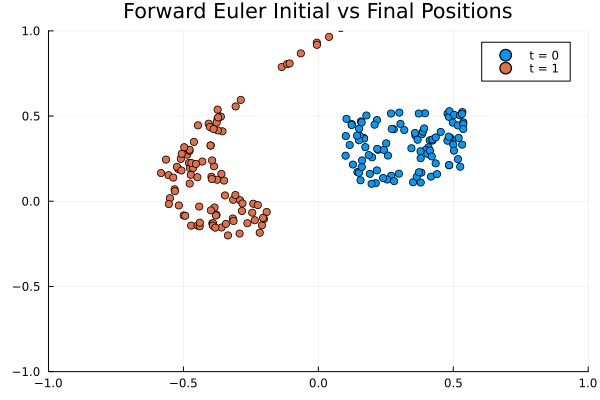
\includegraphics[width=4in]{FE_1_second_solution.png}
  \caption{Initial and final particle positions for 1 second time frame using Forward Euler solver.}
  \label{fig:FE1}
\end{figure}

\begin{figure}[h!]
  \centering
  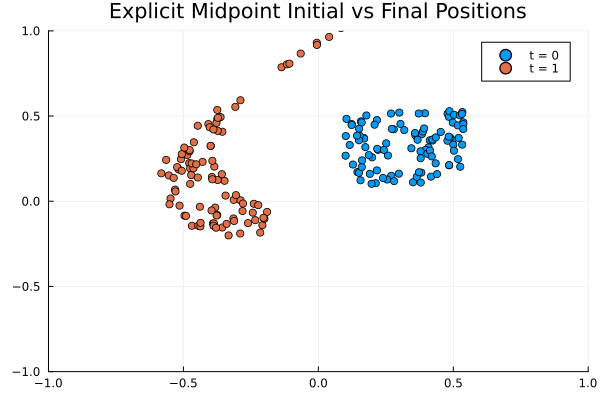
\includegraphics[width=4in]{EM_1_second_solution.png}
  \caption{Initial and final particle positions for 1 second time frame using Explicit Midpoint solver.}
  \label{fig:EM1}
\end{figure}

Figure \ref{fig:EvT} displays the error of both methods at different time steps. The error is defined as the difference in position at time = 5 from the particle positions at time = 0. With the velocities given in Equation \ref{eq:velocity} below, the particle positions at time = 0, should be the same at time = 5. First, take note that as the time step size decreases, the error of both methods decrease. Additionally, it is seen that the Explicit Midpoint method produces results with lower errors.

\begin{equation*}
  \label{eq:velocity}
  \begin{split}
    & v_x(x, y, t) = -\sin (\pi y) \cos (\pi t/C) \\
    & v_y(x, y, t) = \sin (\pi x) \cos (\pi t/C)
  \end{split}
\end{equation*}

\begin{figure}[h!]
  \centering
  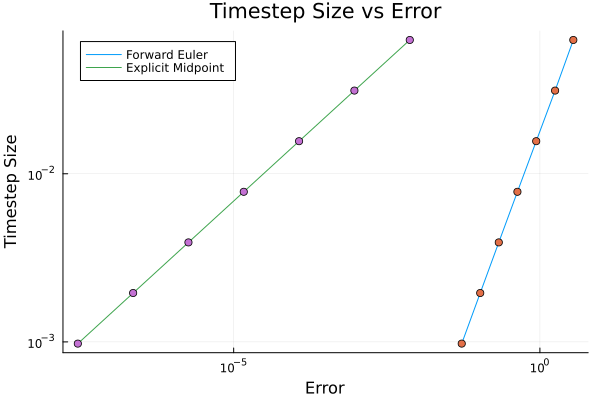
\includegraphics[width=4.6in]{Timestep Size vs Error.png}
  \caption{Solution error at varying time-steps.}
  \label{fig:EvT}
\end{figure}

\section{Analysis of The Efficiency of The "rhs!" Function}

Listing \ref{code1} shows the command to check the type stability of the \jlinl{rhs!} function using \jlinl{@code_warntype}. As shown in Listing \ref{code2}, \jlinl{rhs!} is type stable.

{\LARGE
\begin{jllisting}[caption={Type stable check command.}, label=code1]
num_particles = 100 # number of particles used in simulation
du = zeros(2, num_particles) # array for storing velocity of particles, initialized to zero
u = 0.1 .+ 0.45 * rand(2, num_particles) # intitial position of particles
parameters = [5] # parameter for specified velocity field
t = 1.324 # randomly chosen point in time
@code_warntype rhs!(du, u, parameters, t) # testing type stability with a representative set of inputs defined above
\end{jllisting}
}

{\LARGE
\begin{jllisting}[caption={Type stable check output.}, label=code2]
MethodInstance for rhs!(::Matrix{Float64}, ::Matrix{Float64}, ::Vector{Int64}, ::Float64)
  from rhs!(du, u, parameters, t) in Main at c:\Users\lamki\OneDrive - Rice University\1st Semester\CAAM 519\caam-419-519-submissions\homework-2\part_2.jl:1
Arguments
  #self#::Core.Const(rhs!)
  du::Matrix{Float64}
  u::Matrix{Float64}
  parameters::Vector{Int64}
  t::Float64
Locals
  @_6::Union{Nothing, Tuple{Int64, Int64}}
  N::Int64
  C::Int64
  i::Int64
Body::Nothing
\end{jllisting}
}

Listing \ref{code3} shows the command to check the speed of the \jlinl{rhs!} function using \jlinl{@btime}. This command also checks how many allocations the function uses. As shown in Listing \ref{code4}, \jlinl{rhs!} is allocation-free.

{\LARGE
\begin{jllisting}[caption={Type stable check command.}, label=code3]
num_particles = 100 # number of particles used in simulation
du = zeros(2, num_particles) # array for storing velocity of particles, initialized to zero
u = 0.1 .+ 0.45 * rand(2, num_particles) # intitial position of particles
parameters = [5] # parameter for specified velocity field
t = 1.324 # randomly chosen point in time
@btime rhs!($du, $u, $parameters, $t)
\end{jllisting}
}

{\LARGE
\begin{jllisting}[caption={Type stable check output.}, label=code4]
4.400 μs (0 allocations: 0 bytes)
\end{jllisting}
}

\section{Analysis of The Efficiency of The Solver Functions}

Listing \ref{code5} shows the command to check the type stability of the \jlinl{solve} function using \jlinl{@code_warntype}. As shown in Listing \ref{code6}, \jlinl{solve} is type stable.

{\LARGE
\begin{jllisting}[caption={Type stable check command.}, label=code5]
num_particles = 100 # number of particles used in simulation
u = 0.1 .+ 0.45 * rand(2, num_particles) # intitial position of particles
tspan = (0, 5) # randomly chosen time span
dt = 1/512 # randomly chosen time step
parameters = [5] # parameter for specified velocity field
@code_warntype solve(ForwardEuler(), u, rhs!, tspan, dt, parameters)
\end{jllisting}
}

{\LARGE
\begin{jllisting}[caption={Type stable check output.}, label=code6]
MethodInstance for solve(::ForwardEuler, ::Matrix{Float64}, ::typeof(rhs!), ::Tuple{Int64, Int64}, ::Float64, ::Vector{Int64})
  from solve(method::ForwardEuler, u0, rhs!, tspan, dt, parameters; num_saved_steps) in Main at c:\Users\lamki\OneDrive - Rice University\1st Semester\CAAM 519\caam-419-519-submissions\homework-2\part_1.jl:3
Arguments
  #self#::Core.Const(solve)
  method::Core.Const(ForwardEuler())
  u0::Matrix{Float64}
  rhs!::Core.Const(rhs!)
  tspan::Tuple{Int64, Int64}
  dt::Float64
  parameters::Vector{Int64}
Body::Vector{Matrix{Float64}}
\end{jllisting}
}

Figure \ref{fig:EvN} displays the error of both methods at different number of \jlinl{rhs!} evaluations. The error is defined the same way as mentioned previously. The number of \jlinl{rhs!} evaluations is found by the number of times the solve function calls \jlinl{rhs!} during its execution. For a given \jlinl{dt}, the Explicit Midpoint methods calls the \jlinl{rhs!} function double the amount the Forward Euler method calls it. Looking at Figure \ref{fig:EvN}, note that as the number of \jlinl{rhs!} evaluations increases, the error of both methods decrease. Additionally, it is seen that the Explicit Midpoint method produces results with lower errors, similar to what was seen with Figure \ref{fig:EvT}.

\begin{figure}[h!]
  \centering
  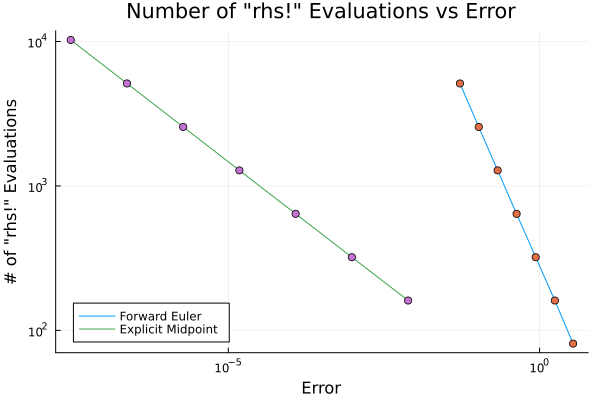
\includegraphics[width=4.6in]{Number of rhs! Evaluations vs Error.png}
  \caption{Solution error at varying number of rhs! evaluations.}
  \label{fig:EvN}
\end{figure}


\end{document}
